
%(BEGIN_QUESTION)
% Copyright 2007, Tony R. Kuphaldt, released under the Creative Commons Attribution License (v 1.0)
% This means you may do almost anything with this work of mine, so long as you give me proper credit

An instrument technician needs to connect one discrete output of a PLC to one discrete input of a DCS.  The problem is, the PLC's output module is intended to switch 120 volt AC power, while the DCS input module can only handle 24 volts DC.  The following schematic shows the internal connections inside each module, complete with the opto-isolators within each:

$$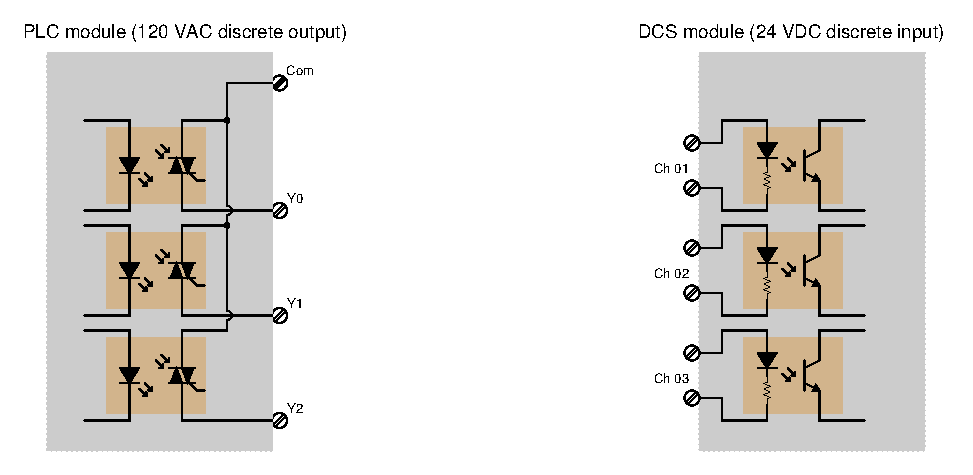
\includegraphics[width=15.5cm]{i02534x01.eps}$$

\vskip 80pt

Sketch an interposing circuit that will allow output channel Y1 of the PLC connect to drive input channel 3 of the DCS.  Be sure to include any necessary power source connections (e.g. L1, Neutral, positive DC, negative DC, etc.) and components to make this work.

\underbar{file i02534}
%(END_QUESTION)





%(BEGIN_ANSWER)

{\it Full credit for a completely correct solution (e.g. PLC energizes an electromechanical relay with a 120 VAC coil, the contacts of that relay sending 24 VDC to the DCS input.}

\vskip 10pt

{\it Half credit for a solution that would work once or twice but not reliably over time (e.g. 120 VAC through a large resistor to the DCS input channel).}

%(END_ANSWER)





%(BEGIN_NOTES)

{\bf This question is intended for exams only and not worksheets!}

%(END_NOTES)


